\documentclass[../main.tex]{subfiles}
\begin{document}
\subsubsection{Deterministic transitions: bifurcation-induced (B-)tipping}\label{subsubsec3.1.1}
In classical dynamical systems, the location (in state space) and the stability of equilibria and their manifolds is studied at fixed values of the parameter $\mu$.
In the context of bifurcation theory in fact the loss of hyperbolicity of these objects may cause the system to undergo a local or global bifurcation which inherently changes the stability or even the existence of the attractors. 
This causes the model's state to shift the dynamical regime from slow stable time-evolution to a fast unstable one.
The theory upon which these systems are investigated has been known since the 1930s\footnote{\url{http://www.scholarpedia.org/article/History\_of\_dynamical\_systems}} and ever since expanded upon to include complex dynamics such as chaos theory and delayed differential equations (DDEs).
However in real-world phenomena it is reasonable to assume that while the system's dynamics dictates the evolution of the observables in phase space at specific parameter values, the system properties also indirectly affect the parameter itself.
Therefore the first assumption to be dropped in our quest of deriving these high-fidelity models is the stationarity of the parameter $\mu$ and the formulation of an augmented (albeit still low-dimensional) version of the original system. 
In the simplest form the time variation of the parameter is monotonic and linear with the ramping characterised by a timescale $\tau:=\varepsilon t$, $0<\varepsilon\ll1$ much slower than that of the observables' dynamics.
The resulting system is therefore called fast-slow
\begin{equation}\label{eq3.1}
   \begin{cases}
           \dot{x}:=\frac{d}{dt}x=f(x;\mu) \,, \\
           \dot{\mu}:=\frac{d}{dt}\mu=\varepsilon \,, 
   \end{cases}\quad \longleftrightarrow\quad
   \begin{cases}
           \newprime{x}:=\frac{d}{d\tau}x=\varepsilon^{-1}f(x;\mu)\,, \\
           \newprime{\mu}:=\frac{d}{d\tau}\mu=1\,,
   \end{cases}
\end{equation}
and it has been the cornerstone object for the development of geometric singular perturbation theory (GSPT) \cite{Wechselberger20}, extensively applied in the analysis of biological mechanisms s.a. calcium cell signaling \cite{Pages19}.
In \cite{Kuehn11} such formulation is the starting point in the discussion of a general and robust framework for the characterisation of critical transitions in low-dimensional systems.
Notably the fast-slow dynamics is approximated by resolving the layer equation
\begin{equation}\label{eq3.2}
   \begin{cases}
           \dot{x}=f(x;\mu) \,, \\
           \dot{\mu}=0 \,, 
   \end{cases}
\end{equation}
which is obtained by taking the singular limit $\varepsilon\to0$ of the system in the fast timescale (i.e. the leftmost system in \eqref{eq3.1}), and the reduced equation
\begin{equation}\label{eq3.3}
   \begin{cases}
      0=f(x;\mu) \,, \\
      \newprime{\mu}=1 \,, 
   \end{cases}
\end{equation}
which is derived via the singular limit of the system in slow timescale (which is the rightmost system in \eqref{eq3.1}).
The centerpiece of the whole analysis is the derivation of the critical manifold $C:=\{(x,\mu)\in \mathbb{R}^{n+m}\;:\;f(x;\mu)=0\}$ as it constraints the solutions of the slow subsystem \eqref{eq3.3} to a unique codim$-m$ object as shown in the example depicted in Figure \ref{fig3.1} below.
An important result from GSPT allows us to characterise a family of (infinitely many) slow manifolds $C_{\varepsilon}:=\{(x,\mu)\in \mathbb{R}^{N+M}\;:\;x=h_{\varepsilon}(\mu)=h(\mu)+\mathcal{O}(\varepsilon)\}$ where $h:\mu\to x$ is given by the Implicit Function Theorem.
\begin{theorem}[label=thm3.1]{Fenichel's $(1^{st})$ Theorem}{}
     Let $C$ be a compact, normally hyperbolic manifold then for $\varepsilon>0$ sufficiently small there exists $C_{\varepsilon}$ locally invariant and diffeomorphic to $C$ that lies at a Hausdorff distance $O(\varepsilon)$ from $C$.
\end{theorem}
These singularly perturbed slow manifolds will become paramount later on in the derivation of statistical measure as precursors of critical transitions which we hereby define.
\begin{definition}[Critical transition]\label{def3.1}
     Let $\gamma(t)$ be a homeomorphic image of the real subset $(a,b)$ s.t. for each partitioning ${a=t_{0}<t_1,\dots,t_{N-1}<t_N=b}$ the image $\gamma(t_{j-1},t_j)$ is an orientation preserving trajectory of either the layer \eqref{eq3.2} or the reduced equation \eqref{eq3.3} and let $p\in C$ be a point where the critical manifold loses its hyperbolicity, then $p$ is a critical transition if there exist a candidate trajectory $\gamma$ s.t. $p = \gamma(t_j)$ is a transition between fast and slow regimes and $\gamma(t_{j-1},t_j)$ is hyperbolic and attracting.
\end{definition}
\begin{figure}[H]
       \centering 
       \begin{subfigure}[b]{0.475\textwidth}
        \centering 
        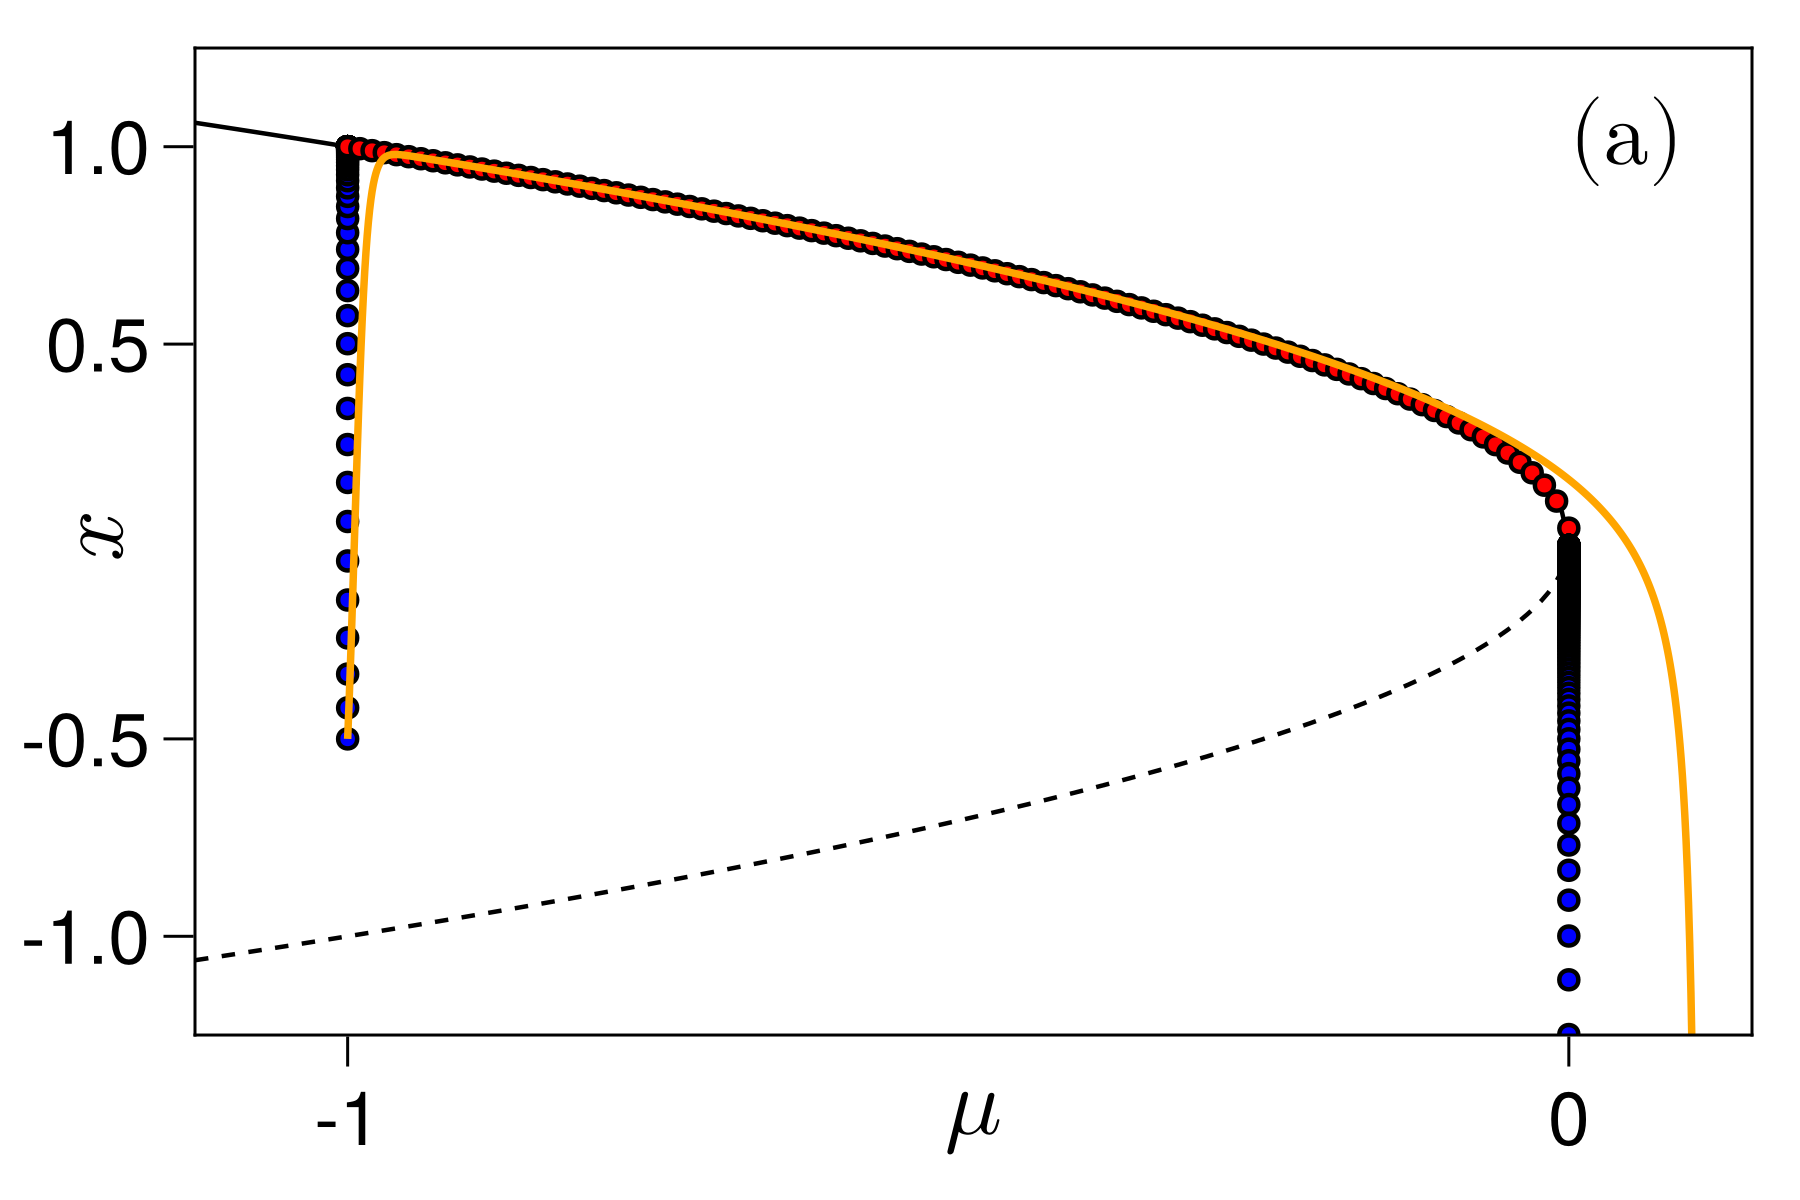
\includegraphics[keepaspectratio, width = \textwidth]{../figures/fig3.1.1.png}
        \label{fig3.1.1}
       \end{subfigure}
       \hfill 
       \begin{subfigure}[b]{0.475\textwidth}
        \centering 
        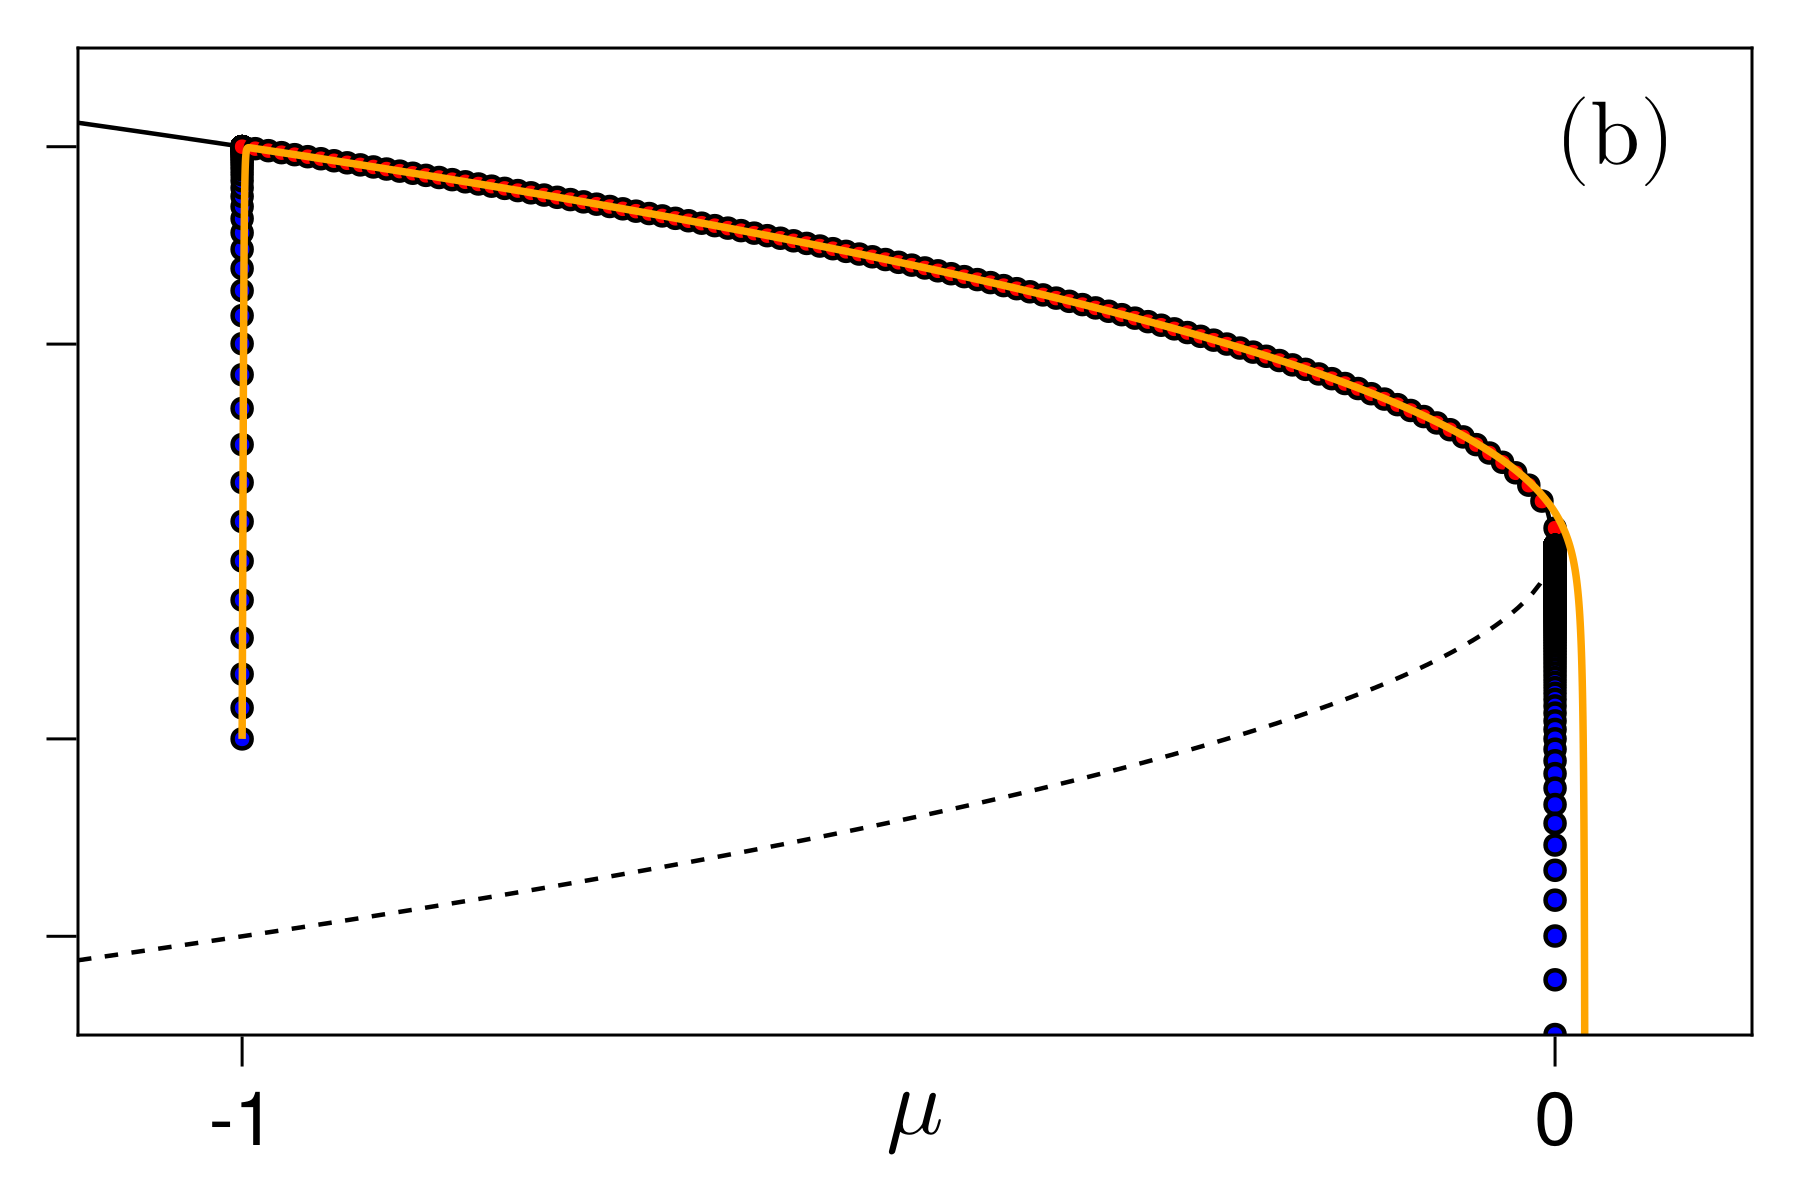
\includegraphics[keepaspectratio, width = \textwidth]{../figures/fig3.1.2.png}
        \label{fig3.1.2}
       \end{subfigure}
       \caption{Comparison of the (numerical) fast-slow trajectory (yellow curve) of the codim$-1$ saddle-node normal form  with different linear rampings ((a): $\varepsilon=10^{-2}$; (b): $\varepsilon=10^{-3}$) and its approximation given by different regimes in the singular limit.
       Solutions of the layer problem \eqref{eq3.2} in blue dots, with initial conditions $(-0.5,-1)$ and $(0,0)$, connected by a solution of the reduced problem \eqref{eq3.3} in red dots with initial condition $(1,-1)$. 
Notice how the dynamics on the critical manifold prescribes the solution of the slow subsystem and the delay of the critical transition in the fast regime is determined by the value of the timescale separation constant $\varepsilon$.}
       \label{fig3.1}
\end{figure}
\end{document}
